%!TEX root = ../thesis.tex
\documentclass[../../thesis.tex]{subfiles}

\begin{document}
\begin{figure}[tb]
    \centering
    \subfloat[]{
    \tikzsetnextfilename{pore_disorder_1}
    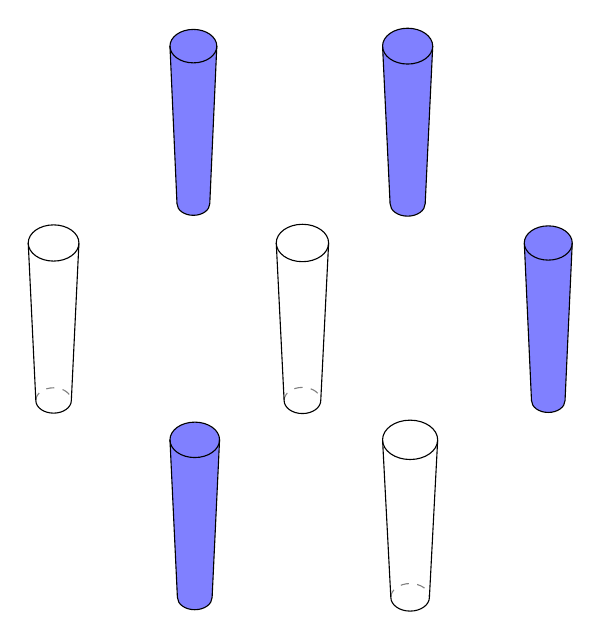
\begin{tikzpicture}
        \pgfdeclarelayer{bg}    % declare background layer
        \pgfdeclarelayer{bbg}    % declare backbackground layer
        \pgfsetlayers{bbg,bg,main}  % set the order of the layers (main is the standard layer)
        \def\height{2}
        \def\primaryRadius{0.35}
        \def\secondaryRadius{.25}
        \def\funneling{0.7}
        \foreach \X/\Y/\F in {1.8/0/0.9, 4.5/0/1, 1.8/5/0.85, 4.5/5/0.91, 3.15/2.5/0.95, 0/2.5/0.92, 6.3/2.5/0.87}
            {
            \draw ({\X + (1 - \funneling) * \primaryRadius * \F}, \Y) arc(180:360:{\funneling * \primaryRadius * \F} and {\funneling * \secondaryRadius * \F}) -- (\X + 2 * \primaryRadius * \F, \Y + \height) arc (0:180:{\primaryRadius * \F} and {\secondaryRadius * \F}) -- cycle;
            \draw (\X + 2 * \primaryRadius * \F, \Y + \height) arc(0:-180: {\primaryRadius * \F} and \secondaryRadius * \F);
            \begin{pgfonlayer}{bbg}
                \draw[dashed, gray] ({\X + (1 - \funneling) * \primaryRadius * \F},\Y) arc(180:0:{\funneling * \primaryRadius * \F} and \funneling * \secondaryRadius * \F);
            \end{pgfonlayer}
            }
        \begin{pgfonlayer}{bg}
            \foreach \X/\Y/\F in {1.8/0/0.9,  1.8/5/0.85, 4.5/5/0.91, 6.3/2.5/0.87}
                {
                \fill[blue!50] ({\X + (1 - \funneling) * \primaryRadius * \F}, \Y) arc(180:360:{\funneling * \primaryRadius * \F} and {\funneling * \secondaryRadius * \F}) -- (\X + 2 * \primaryRadius * \F, \Y + \height) arc (0:180:{\primaryRadius * \F} and {\secondaryRadius * \F}) -- cycle;
                }
        \end{pgfonlayer}
    \end{tikzpicture}
    \label{fig:disorder-absorption}}
    \hfill
    \subfloat[]{
    \tikzsetnextfilename{pore_disorder_2}
    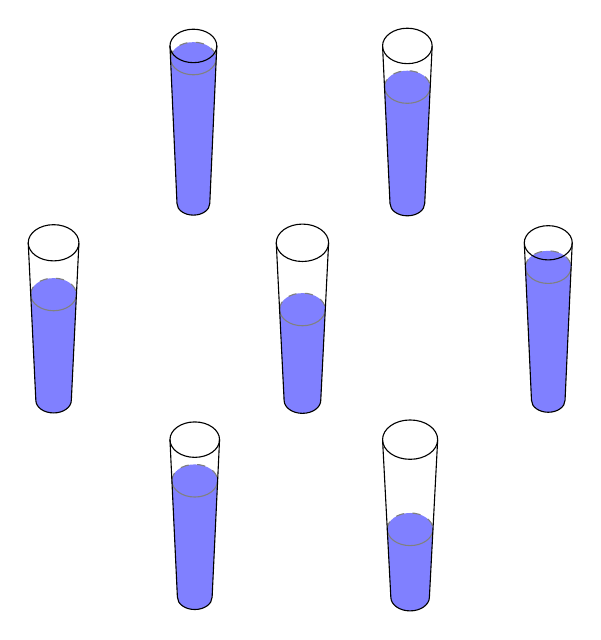
\begin{tikzpicture}
        \pgfdeclarelayer{bg}    % declare background layer
        \pgfdeclarelayer{bbg}    % declare backbackground layer
        \pgfsetlayers{bbg,bg,main}  % set the order of the layers (main is the standard layer)
        \def\height{2}
        \def\primaryRadius{.35}
        \def\secondaryRadius{.25}
        \def\rmax{0.29}
        \def\funneling{0.7}
        \foreach \X/\Y/\F in {1.8/0/0.9, 4.5/0/1, 1.8/5/0.85, 4.5/5/0.9, 3.15/2.5/0.95, 0/2.5/0.92, 6.3/2.5/0.87}
            {
            \draw ({\X + (1 - \funneling) * \primaryRadius * \F}, \Y) arc(180:360:{\funneling * \primaryRadius * \F} and {\funneling * \secondaryRadius * \F}) -- (\X + 2 * \primaryRadius * \F, \Y + \height) arc (0:180:{\primaryRadius * \F} and {\secondaryRadius * \F}) -- cycle;
            \draw (\X + 2 * \primaryRadius * \F, \Y + \height) arc(0:-180: {\primaryRadius * \F} and \secondaryRadius * \F);
            \begin{pgfonlayer}{bbg}
                \draw[dashed, gray] ({\X + (1 - \funneling) * \primaryRadius * \F},\Y) arc(180:0:{\funneling * \primaryRadius * \F} and \funneling * \secondaryRadius * \F);
            \end{pgfonlayer}
            %
            \begin{pgfonlayer}{bg}
                \fill[blue!50] ({\X + \primaryRadius * \F - \rmax}, {\Y + 3.35 * ((\rmax - \F * \funneling * \primaryRadius) * \height / \F / \primaryRadius}) arc(-180:-360:{\rmax} and {\rmax * \secondaryRadius / \primaryRadius}) -- ({\X + (1 - \funneling) * \primaryRadius * \F + 2 * \primaryRadius * \F * \funneling}, \Y) arc (0:-180:{\funneling * \primaryRadius * \F} and {\funneling * \secondaryRadius * \F});
                \draw[gray, dashed, thin] ({\X + \primaryRadius * \F - \rmax}, {\Y + 3.35 * ((\rmax - \F * \funneling * \primaryRadius) * \height / \F / \primaryRadius}) arc(-180:-360:{\rmax} and {\rmax * \secondaryRadius / \primaryRadius});
                \draw[gray, thin] ({\X + \primaryRadius * \F - \rmax}, {\Y + 3.35 * ((\rmax - \F * \funneling * \primaryRadius) * \height / \F / \primaryRadius}) arc(180:360:{\rmax} and {\rmax * \secondaryRadius / \primaryRadius});
            \end{pgfonlayer}
            }
    \end{tikzpicture}
    \label{fig:disorder-desorption}}
    \caption{Disorder between neighboring pores during absorption \protect\subref{fig:disorder-absorption} and desorption \protect\subref{fig:disorder-desorption}. Important is the larger degree of disorder upon the absorption process. Upon condensation pores fill immediately when the spinodal pressure $P_\mathrm{sp}(d_\mathrm{min})$ is reached, where $d_\mathrm{min}$ is the radius of the opening at the small end. The evaporation is continuous at equilibrium pressure $P_\mathrm{eq}(d)$ and empties each pore simultaneously while the diameter $d$ is large enough.}
    \label{fig:pore-disorder}
\end{figure}


\end{document}
